\section{Our Mining Framework for Ethereum}\label{sec:mining-ethereum-algorithm} 

We start this section with a high-level overview of our algorithm and then provide the details of each step. The fundamental idea behind our approach is a simple observation: in real-world instances of the problem, each transaction interacts with only a few other transactions, which we call its neighborhood. Thus, when forming a block, we do not need to search over all possible permutations of transactions, but can instead find rules that encode the gas usage of each transaction based on the portion of its neighborhood that precedes it in the block.

\paragraph{Overview} Our approach consists of the following steps:
\begin{enumerate}
	\item \emph{Sampling and Testing.} We start by sampling random permutations of the transactions available in our $\pool$ and executing them, keeping track of the amount of gas used by each transaction in each sample permutation.
	\item \emph{Neighborhood Estimation.} For each transaction $\tx,$ we identify a neighborhood, i.e.~a set $\nbhd(\tx)$ of transactions whose inclusion before $\tx$ has the potential to change the amount of gas consumed by $\tx.$ To estimate each transaction's neighborhood, we rely on a decision tree generated from our samples.
	\item \emph{Extracting Gas Usage Rules.} Using the neighborhoods and samples, we extract gas usage rules.  We define a simple grammar that can encode rules such as ``if $\tx_1$ appears before $\tx_2$ which in turn appears before $\tx_3,$ then $\tx_3$ will have a gas usage of $g$'' for $\tx_1, \tx_2 \in \nbhd(\tx_3).$ We show that such rules can be mined from our samples, using a different decision tree.
	\item \emph{Translating Gas Usage Rules to ILP.} Our goal is to obtain a block that orders a subset of transactions in a manner that maximizes the total tip earned by the miner. To do this, we have to choose which rules from the previous step to follow, i.e. which local orderings to include, but cannot choose rules that require conflicting orders on the transactions. Our algorithm translates this problem to integer linear programming (ILP).
	\item \emph{Solving the ILP.} Finally, we call an external off-the-shelf ILP-solver to handle the ILP instance generated in the previous step. This yields the desired block. 
\end{enumerate}



\paragraph{Step (1): Sampling and Testing}
The input to our algorithm is the initial world state $s_0$ and a set $\pool = \{ \tx_1, \tx_2, \ldots, \tx_n \}$ of valid transactions which are not yet added to the blockchain. In this step, we randomly and uniformly generate several permutations $\Pi = \{\pi_1, \pi_2, \ldots, \pi_k\}$ of our $\pool.$ The number of samples, $k,$ is a user-defined parameter. Note that the $\pi_i$'s are not necessarily valid blocks as they might exceed the block gas limit.

% Question: Does this mean that we removed faulty transactions for orders?
We need to perform some simple housekeeping at this point. Recall that transactions originating from the same account should appear in the order of their nonces. We say a transaction $\tx$ is an $a$-transaction if it originates from an account with address $a.$ For every $i$ and $a,$ we sort all the $a$-transactions in $\pi_i$ by their nonce, thus ensuring that every sample $\pi_i$ respects nonce orders. If there are several $a$-transactions with the same nonce in $\pi_i$, we only keep the first and remove the rest. Thus, $\pi_i$ might end up containing only a subset of the transactions in $\pool.$

We then execute every sample $\pi_i$ starting from the initial world state $s_0$ and keep track of the amount of gas used by each transaction $\tx_j$ in the execution of $\pi_i.$ We denote this by $\gas(\pi_i, \tx_j).$


\paragraph{Example} Suppose we have 6 transactions in our pool and the tip value set by the users is $t[\tx_1, \tx_2, \tx_3,  \tx_4,  \tx_5,  \tx_6] = [24, 9, 5, 29, 24, 2],$ i.e.~$\tx_1$ pays a tip of $24$ for each consumed unit of gas, $\tx_2$ pays $9,$ etc. We generate $k=10$ random permutations $\pi_1, \ldots, \pi_{10}$ of the pool, execute them, and keep track of the gas used by each transaction in each sample.  See Figure~\ref{fig:mining-ethereum-fuzzing}.


\paragraph{Step (2): Neighborhood Estimation} In this step, we consider each transaction $\tx_i \in \pool$ separately and our goal is to identify a neighborhood for it, i.e.~a set of transactions $\nbhd(\tx_i) \subseteq \pool$ whose inclusion before $\tx_i$ can potentially change the amount of gas consumed by $\tx_i.$ We observe that the transactions usually exhibit only a few different possible gas usage values. Thus, we can use the amount of gas used by $\tx_i$ as a label in a classification problem. We introduce one binary attribute for each $\tx_j,$ which is set to $1$ if $\tx_j$  precedes $\tx_i$ in the sample permutation. We then generate a decision tree. At each node of the tree, we choose the best possible attribute to branch on, based on the Gini impurity metric \cite[Chapter 4.6]{breiman1984classification}. After generating the decision tree, if the attribute corresponding to $\tx_j$ appears in one of the decisions, we add $\tx_j$ to the neighborhood $\nbhd(\tx_i).$

\paragraph{Example} Consider the samples of the previous example (Figure~\ref{fig:mining-ethereum-fuzzing}). In this step, our algorithm finds a neighborhood for every transaction. Let us consider $\tx_3.$ We can encode each permutation $\pi_i$ as a vector $v_i$ such that $v_i[j] = 1$ if $\tx_j$ precedes $\tx_3$ in $\pi_i$ and $v_i[j]=0$ otherwise. The label associated with $v_i$ is the gas usage of $\tx_3$ in the execution of $\pi_i.$ In this case, there are only two possible labels: $2$ and $4$. See Figure~\ref{fig:mining-ethereum-dectree} (left). When we generate a decision tree, shown in Figure~\ref{fig:mining-ethereum-dectree} (right), it only looks at the attribute corresponding to $\tx_2.$ Hence, we set $\nbhd(\tx_3) = \{\tx_2\}.$ In other words, at least in our samples, the gas usage of $\tx_3$ is only dependent on whether $\tx_2$ precedes it. This is shown in Figure~\ref{fig:mining-ethereum-nei}.


\begin{figure}[!p]
\centering
\begin{tikzpicture}[scale=1.5, transform shape, every node/.style={font=\small}]
	% Permutation deabcf: 554 gas: [2, 10, 6, 8, 4, 10] (sum: 40) fees: [58, 240, 144, 72, 20, 20] (sum: 554)
	\def\row{0}
	\def\col{0}
	\txheader{(0 + \col)}{\row}
	\txd   {2}   {58 } {(1 + \col)}{\row}
	\txe  {10}  {240 } {(2 + \col)}{\row}
	\txa   {6}  {144 } {(3 + \col)}{\row}
	\txb   {8}   {72 } {(4 + \col)}{\row}
	\txc   {4}   {20 } {(5 + \col)}{\row}
	\txf  {10}   {20 } {(6 + \col)}{\row}
	\txres{1}{40}  {554 } {(7 + \col)}{\row}
	
	% Permutation bdacef: 410 gas: [8, 2, 8, 4, 2, 10] (sum: 34) fees: [72, 58, 192, 20, 48, 20] (sum: 410)
	\def\row{0}
	\def\col{7.5}
	% \txheader{(0 + \col)}{\row}
	\txb{ 8}{ 72 }{(1 + \col)}{\row}
	\txd{ 2}{ 58 }{(2 + \col)}{\row}
	\txa{ 8}{192 }{(3 + \col)}{\row}
	\txc{ 4}{ 20 }{(4 + \col)}{\row}
	\txe{ 2}{ 48 }{(5 + \col)}{\row}
	\txf{10}{ 20 }{(6 + \col)}{\row}
	\txres{2}{34}{410 }{(7 + \col)}{\row}
\end{tikzpicture}

\begin{tikzpicture}[scale=1.5, transform shape, every node/.style={font=\small}]
	% Permutation bcfaed: 506 gas: [8, 4, 10, 10, 4, 2] (sum: 38) fees: [72, 20, 20, 240, 96, 58] (sum: 506)
	\def\row{0}
	\def\col{0}
	\txheader{(0 + \col)}{\row}
	\txb{8}{72 }{(1 + \col)}{\row}
	\txc{4}{20 }{(2 + \col)}{\row}
	\txf{10}{20 }{(3 + \col)}{\row}
	\txa{10}{240 }{(4 + \col)}{\row}
	\txe{4}{96 }{(5 + \col)}{\row}
	\txd{2}{58 }{(6 + \col)}{\row}
	\txres{3}{38}{506 }{(7 + \col)}{\row}
	
	
	% Permutation dacfeb: 601 gas: [2, 8, 2, 10, 10, 9] (sum: 41) fees: [58, 192, 10, 20, 240, 81] (sum: 601)
	\def\row{0}
	\def\col{7.5}
	% \txheader{(0 + \col)}{\row}
	\txd{2}{58 }{(1 + \col)}{\row}
	\txa{8}{192 }{(2 + \col)}{\row}
	\txc{2}{10 }{(3 + \col)}{\row}
	\txf{10}{20 }{(4 + \col)}{\row}
	\txe{10}{240 }{(5 + \col)}{\row}
	\txb{9}{81 }{(6 + \col)}{\row}
	\txres{4}{41}{601 }{(7 + \col)}{\row}
\end{tikzpicture}

\begin{tikzpicture}[scale=1.5, transform shape, every node/.style={font=\small}]
	% Permutation dfeabc: 553 gas: [2, 5, 10, 6, 9, 4] (sum: 36) fees: [58, 10, 240, 144, 81, 20] (sum: 553)
	\def\row{0}
	\def\col{0}
	\txheader{(0 + \col)}{\row}
	\txd{2}{58 }{(1 + \col)}{\row}
	\txf{5}{10 }{(2 + \col)}{\row}
	\txe{10}{240 }{(3 + \col)}{\row}
	\txa{6}{144 }{(4 + \col)}{\row}
	\txb{9}{81 }{(5 + \col)}{\row}
	\txc{4}{20 }{(6 + \col)}{\row}
	\txres{5}{36}{553 }{(7 + \col)}{\row}
	
	% Permutation fdcbae: 591 gas: [5, 2, 2, 9, 8, 10] (sum: 36) fees: [10, 58, 10, 81, 192, 240] (sum: 591)
	
	\def\row{0}
	\def\col{7.5}
	% \txheader{(0 + \col)}{\row}
	\txf{5}{10 }{(1 + \col)}{\row}
	\txd{2}{58 }{(2 + \col)}{\row}
	\txc{2}{10 }{(3 + \col)}{\row}
	\txb{9}{81 }{(4 + \col)}{\row}
	\txa{8}{192 }{(5 + \col)}{\row}
	\txe{10}{240 }{(6 + \col)}{\row}
	\txres{6}{36}{591 }{(7 + \col)}{\row}
\end{tikzpicture}

\begin{tikzpicture}[scale=1.5, transform shape, every node/.style={font=\small}]
	% Permutation efacdb: 447 gas: [10, 5, 2, 2, 2, 9] (sum: 30) fees: [240, 10, 48, 10, 58, 81] (sum: 447)
	\def\row{0}
	\def\col{0}
	\txheader{(0 + \col)}{\row}
	\txheader{(0 + \col)}{\row}
	\txe{10}{240 }{(1 + \col)}{\row}
	\txf{5}{10 }{(2 + \col)}{\row}
	\txa{2}{48 }{(3 + \col)}{\row}
	\txc{2}{10 }{(4 + \col)}{\row}
	\txd{2}{58 }{(5 + \col)}{\row}
	\txb{9}{81 }{(6 + \col)}{\row}
	\txres{7}{30}{447 }{(7 + \col)}{\row}  
	
	
	% Permutation adecbf: 640 gas: [10, 2, 10, 2, 8, 10] (sum: 42) fees: [240, 58, 240, 10, 72, 20] (sum: 640)
	\def\row{0}
	\def\col{7.5}
	% \txheader{(0 + \col)}{\row}
	\txa{10}{240 }{(1 + \col)}{\row}
	\txd{2}{58 }{(2 + \col)}{\row}
	\txe{10}{240 }{(3 + \col)}{\row}
	\txc{2}{10 }{(4 + \col)}{\row}
	\txb{8}{72 }{(5 + \col)}{\row}
	\txf{10}{20 }{(6 + \col)}{\row}
	\txres{8}{42}{640 }{(7 + \col)}{\row}
\end{tikzpicture}

\begin{tikzpicture}[scale=1.5, transform shape, every node/.style={font=\small}]
	% Permutation cfbead: 313 gas: [2, 10, 9, 4, 2, 2] (sum: 29) fees: [10, 20, 81, 96, 48, 58] (sum: 313)
	\def\row{0}
	\def\col{0}
	\txheader{(0 + \col)}{\row}
	\txc{2}{10 }{(1 + \col)}{\row}
	\txf{10}{20 }{(2 + \col)}{\row}
	\txb{9}{81 }{(3 + \col)}{\row}
	\txe{4}{96 }{(4 + \col)}{\row}
	\txa{2}{48 }{(5 + \col)}{\row}
	\txd{2}{58 }{(6 + \col)}{\row}
	\txres{9}{29}{313 }{(7 + \col)}{\row}
	
	% Permutation bacedf: 506 gas: [8, 10, 4, 4, 2, 10] (sum: 38) fees: [72, 240, 20, 96, 58, 20] (sum: 506)
	\def\row{0}
	\def\col{7.5}
	% \txheader{(0 + \col)}{\row}
	\txb{8}{72 }{(1 + \col)}{\row}
	\txa{10}{240 }{(2 + \col)}{\row}
	\txc{4}{20 }{(3 + \col)}{\row}
	\txe{4}{96 }{(4 + \col)}{\row}
	\txd{2}{58 }{(5 + \col)}{\row}
	\txf{10}{20 }{(6 + \col)}{\row}
	\txres{10}{38}{506 }{(7 + \col)}{\row}
\end{tikzpicture}
\caption{An example execution of $10$ samples of a pool of $6$ transactions, profiling the gas usage and tip revenue obtained from each transaction.} 
\label{fig:mining-ethereum-fuzzing}
\end{figure}

\begin{figure}[!p]
\centering
\begin{tikzpicture}[scale=1.5, transform shape, every node/.style={font=\small}]
	% Permutation deabcf: 554 gas: [2, 10, 6, 8, 4, 10] (sum: 40) fees: [58, 240, 144, 72, 20, 20] (sum: 554)
	\def\row{0}
	\def\col{0}
	\txheader{(0 + \col)}{\row}
	\txdOff   {2}   {58 } {(1 + \col)}{\row}
	\txeOff  {10}  {240 } {(2 + \col)}{\row}
	\txaOff   {6}  {144 } {(3 + \col)}{\row}
	\txbN   {8}   {72 } {(4 + \col)}{\row}
	\txcOn   {4}   {20 } {(5 + \col)}{\row}
	\txfOff  {10}   {20 } {(6 + \col)}{\row}
	
	% Permutation bdacef: 410 gas: [8, 2, 8, 4, 2, 10] (sum: 34) fees: [72, 58, 192, 20, 48, 20] (sum: 410)
	\def\row{0}
	\def\col{7}
	% \txheader{(0 + \col)}{\row}
	\txbN{ 8}{ 72 }{(1 + \col)}{\row}
	\txdOff{ 2}{ 58 }{(2 + \col)}{\row}
	\txaOff{ 8}{192 }{(3 + \col)}{\row}
	\txcOn{ 4}{ 20 }{(4 + \col)}{\row}
	\txeOff{ 2}{ 48 }{(5 + \col)}{\row}
	\txfOff{10}{ 20 }{(6 + \col)}{\row}
\end{tikzpicture}

\begin{tikzpicture}[scale=1.5, transform shape, every node/.style={font=\small}]
	% Permutation bcfaed: 506 gas: [8, 4, 10, 10, 4, 2] (sum: 38) fees: [72, 20, 20, 240, 96, 58] (sum: 506)
	\def\row{0}
	\def\col{0}
	\txheader{(0 + \col)}{\row}
	\txbN{8}{72 }{(1 + \col)}{\row}
	\txcOn{4}{20 }{(2 + \col)}{\row}
	\txfOff{10}{20 }{(3 + \col)}{\row}
	\txaOff{10}{240 }{(4 + \col)}{\row}
	\txeOff{4}{96 }{(5 + \col)}{\row}
        	\txdOff{2}{58 }{(6 + \col)}{\row}
	
	
	% Permutation dacfeb: 601 gas: [2, 8, 2, 10, 10, 9] (sum: 41) fees: [58, 192, 10, 20, 240, 81] (sum: 601)
	\def\row{0}
	\def\col{7}
	% \txheader{(0 + \col)}{\row}
	\txdOff{2}{58 }{(1 + \col)}{\row}
	\txaOff{8}{192 }{(2 + \col)}{\row}
	\txcOn{2}{10 }{(3 + \col)}{\row}
	\txfOff{10}{20 }{(4 + \col)}{\row}
	\txeOff{10}{240 }{(5 + \col)}{\row}
	\txbN{9}{81 }{(6 + \col)}{\row}
\end{tikzpicture}

\begin{tikzpicture}[scale=1.5, transform shape, every node/.style={font=\small}]
	% Permutation dfeabc: 553 gas: [2, 5, 10, 6, 9, 4] (sum: 36) fees: [58, 10, 240, 144, 81, 20] (sum: 553)
	\def\row{0}
	\def\col{0}
	\txheader{(0 + \col)}{\row}
	\txdOff{2}{58 }{(1 + \col)}{\row}
	\txfOff{5}{10 }{(2 + \col)}{\row}
	\txeOff{10}{240 }{(3 + \col)}{\row}
	\txaOff{6}{144 }{(4 + \col)}{\row}
	\txbN{9}{81 }{(5 + \col)}{\row}
	\txcOn{4}{20 }{(6 + \col)}{\row}
	
	% Permutation fdcbae: 591 gas: [5, 2, 2, 9, 8, 10] (sum: 36) fees: [10, 58, 10, 81, 192, 240] (sum: 591)
	
	\def\row{0}
	\def\col{7}
	% \txheader{(0 + \col)}{\row}
	\txfOff{5}{10 }{(1 + \col)}{\row}
	\txdOff{2}{58 }{(2 + \col)}{\row}
	\txcOn{2}{10 }{(3 + \col)}{\row}
	\txbN{9}{81 }{(4 + \col)}{\row}
	\txaOff{8}{192 }{(5 + \col)}{\row}
	\txeOff{10}{240 }{(6 + \col)}{\row}
\end{tikzpicture}

\begin{tikzpicture}[scale=1.5, transform shape, every node/.style={font=\small}]
	% Permutation efacdb: 447 gas: [10, 5, 2, 2, 2, 9] (sum: 30) fees: [240, 10, 48, 10, 58, 81] (sum: 447)
	\def\row{0}
	\def\col{0}
	\txheader{(0 + \col)}{\row}
	\txheader{(0 + \col)}{\row}
	\txeOff{10}{240 }{(1 + \col)}{\row}
	\txfOff{5}{10 }{(2 + \col)}{\row}
	\txaOff{2}{48 }{(3 + \col)}{\row}
	\txcOn{2}{10 }{(4 + \col)}{\row}
	\txdOff{2}{58 }{(5 + \col)}{\row}
	\txbN{9}{81 }{(6 + \col)}{\row}
	
	
	% Permutation adecbf: 640 gas: [10, 2, 10, 2, 8, 10] (sum: 42) fees: [240, 58, 240, 10, 72, 20] (sum: 640)
	\def\row{0}
	\def\col{7}
	% \txheader{(0 + \col)}{\row}
	\txaOff{10}{240 }{(1 + \col)}{\row}
	\txdOff{2}{58 }{(2 + \col)}{\row}
	\txeOff{10}{240 }{(3 + \col)}{\row}
	\txcOn{2}{10 }{(4 + \col)}{\row}
	\txbN{8}{72 }{(5 + \col)}{\row}
	\txfOff{10}{20 }{(6 + \col)}{\row}
\end{tikzpicture}

\begin{tikzpicture}[scale=1.5, transform shape, every node/.style={font=\small}]
	% Permutation cfbead: 313 gas: [2, 10, 9, 4, 2, 2] (sum: 29) fees: [10, 20, 81, 96, 48, 58] (sum: 313)
	\def\row{0}
	\def\col{0}
	\txheader{(0 + \col)}{\row}
	\txcOn{2}{10 }{(1 + \col)}{\row}
	\txfOff{10}{20 }{(2 + \col)}{\row}
	\txbN{9}{81 }{(3 + \col)}{\row}
	\txeOff{4}{96 }{(4 + \col)}{\row}
	\txaOff{2}{48 }{(5 + \col)}{\row}
	\txdOff{2}{58 }{(6 + \col)}{\row}
	
	% Permutation bacedf: 506 gas: [8, 10, 4, 4, 2, 10] (sum: 38) fees: [72, 240, 20, 96, 58, 20] (sum: 506)
	\def\row{0}
	\def\col{7}
	% \txheader{(0 + \col)}{\row}
	\txbN{8}{72 }{(1 + \col)}{\row}
	\txaOff{10}{240 }{(2 + \col)}{\row}
	\txcOn{4}{20 }{(3 + \col)}{\row}
	\txeOff{4}{20 }{(4 + \col)}{\row}
	\txdOff{2}{58 }{(5 + \col)}{\row}
	\txfOff{10}{20 }{(6 + \col)}{\row}
\end{tikzpicture}
\caption{The gas usage of $\tx_3$ only depends on whether $\tx_2$ preceded it in the sample permutation.}
\label{fig:mining-ethereum-nei}

\end{figure}


\begin{figure}[h]
\centering
\begin{minipage}{0.48\textwidth}
\centering
\begin{tabular}{|c|c|c|}
    \hline
    Sample ($\pi_i$) & Encoding ($v_i$) & Label ($\gamma_3$)\\ \hline\hline
    $\pi_1$ & $[1, 1, 0, 1, 1, 0]$ &  $4$ \\
    $\pi_2$ & $[1, 1, 0, 1, 0, 0]$ &  $4$ \\
    $\pi_3$ & $[0, 1, 0, 0, 0, 0]$ &  $4$ \\
    $\pi_4$ & $[1, 0, 0, 1, 0, 0]$ &  $2$ \\
    $\pi_5$ & $[1, 1, 0, 1, 1, 1]$ &  $4$ \\
    $\pi_6$ & $[0, 0, 0, 1, 0, 1]$ &  $2$ \\
    $\pi_7$ & $[1, 0, 0, 0, 1, 1]$ &  $2$ \\
    $\pi_8$ & $[1, 0, 0, 1, 1, 0]$ &  $2$ \\
    $\pi_9$ & $[0, 0, 0, 0, 0, 0]$ & $2$ \\
    $\pi_{10}$ & $[1, 1, 0, 0, 0, 0]$ &  $4$ \\ 
    \hline
\end{tabular}
\end{minipage}
\hfill
\begin{minipage}{0.48\textwidth}
\centering
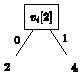
\includegraphics[scale=2.5]{chapters/mining/mining-ethereum-figures/dectree.pdf}
\end{minipage}
\caption{The classification problem is based on the gas used by $\tx_3$ (left) and the resulting decision tree (right).} 
\label{fig:mining-ethereum-dectree}
\end{figure}


\paragraph{Step (3): Extracting Gas Usage Rules} Now that we have estimated the neighborhood of every transaction, our next goal is to extract a set of rules that define the gas usage of each transaction $\tx$ based on the subset of neighbors that precede $\tx$ in the block and their order of appearance.


\paragraph{Syntax} Our rules are defined by the grammar below:
\begin{equation} \label{eq:ethereum-mining-grammar}
\begin{matrix*}[l]
\langle \text{predicate} \rangle & :=  &   \has \tx ~|~  \tx \before \tx ~|~ \neg \langle \text{predicate} \rangle \\
\langle \text{predicate-list} \rangle & :=  & \langle \text{predicate} \rangle ~|~ \langle \text{predicate} \rangle, \langle \text{predicate-list} \rangle    \\
\langle \text{clause} \rangle  & := &  \langle \text{predicate} \rangle ~|~  \atleast(k, \langle \text{predicate-list} \rangle) ~|~\\
& &  \langle \text{clause} \rangle \land \langle \text{clause} \rangle \\
\langle \text{rule} \rangle & := & \langle \text{clause} \rangle  \Rightarrow \expgas(\tx) = g\\
& &g, k \in \mathbb N, \tx \in \pool
\end{matrix*}
\end{equation}



\paragraph{Semantics} Given a sequence of distinct transactions $\pi = \langle \pi[1], \ldots, \pi[m]\rangle, $ we have:
\begin{equation} \label{eq:ethereum-mining-semantics}
\begin{matrix*}[l]
	\pi \models \has\tx_i & \Leftrightarrow & \exists i' ~~ (\pi[i'] = \tx_i) \\
	 \pi \models \tx_i \before \tx_j & \Leftrightarrow & \pi \not\models \has\tx_j \lor \exists i', j' ~~ (i'<j' \land  \\
	 &&\pi[i'] = \tx_i \land \pi[j'] = \tx_j)\\

	 \pi \models \neg p & \Leftrightarrow & \pi \not\models p\\
	 \pi \models c_1 \land c_2 & \Leftrightarrow & \pi \models c_1 \land \pi \models c_2\\
	 \pi \models \atleast(k, p_1, \ldots, p_m) & \Leftrightarrow & \exists i_1, \ldots, i_k ~~ (1 \leq i_1 < \ldots < i_k \leq m \land \\
	 &&\forall j ~~ \pi \models p_{i_j})
\end{matrix*}
\end{equation}

Intuitively, $\pi$ satisfies the predicate $\has \tx_i$ if it includes $\tx_i.$ It satisfies the predicate $\tx_i \before \tx_j$ if it either excludes $\tx_j$ altogether or has $\tx_i$ preceding $\tx_j.$ A clause is simply a conjunction of predicates. We also allow clauses of the form $\atleast(k, p_1, \ldots, p_m)$ which require $\pi$ to satisfy at least $k$ of the predicates $p_1, \ldots, p_m.$ Although the latter could be left as syntactic sugar, including it as a separate clause is helpful in practice. This is because of a common scenario in smart contracts, especially those modeling NFT or token giveaways, in which the first $k$ transactions to call a function can receive the token. In such cases, all transactions calling this function are dependent in terms of gas, but the gas usage of each of them is only dependent on how many other transactions precede it.  Finally, a rule of the form $C \Rightarrow \expgas(\tx_i) \geq g$ signifies a prediction: if $C$ is satisfied, we expect the gas usage of the transaction $\tx_i$ to be at least $g.$



\paragraph{Step (3.i): Generating a Decision Tree}  In this step, we generate a set of rules for each transaction $\tx_i \in \pool.$ We process each such transaction separately. When generating the rules for $\tx_i,$ we narrow our focus down to its neighborhood $\nbhd(\tx_i)$ since we believe these are the only transactions that can affect the gas usage of $\tx_i.$ Let $\pi_j$ be one of the sample permutations. We define $\pi_j^*$ as the subsequence of $\pi_j$ induced by $\nbhd(\tx_i) \cup \{\tx_i\},$ i.e.~the subsequence obtained by removing every element that is not in the neighborhood or not $\tx_i$ itself. If $\pi \not\models \has \tx_i,$ we ignore this sample as it does not include $\tx_i$ and cannot give us any information about its gas usage. We use $\Pi^*$ to denote the set of neighborhood-induced samples.
 
 As in Step 2, our goal is to form a decision tree that predicts the gas usage of $\tx_i$ based on features that encode the set of neighbors that precede it in the block and their order. Thus, for every neighboring $\tx_j \in \nbhd(\tx_i)$ we define a corresponding feature
 $$
 w[j] = \left\{ 
 	\begin{matrix}
 		j' - i' &  \text{if }\pi^* \models \tx_j \before \tx_i \land \pi^*[i']=\tx_i  \land \pi^*[j'] = \tx_j \\
 		0 & \text{otherwise}
 	\end{matrix}
 	\right..
 $$   
 Informally, if $\pi^*$ puts $\tx_j$ before $\tx_i,$ then $-w[j]$ is the distance between the two transactions in $\pi^*.$ Otherwise, $w[j]=0.$ In other words, we care about the distance only if $\tx_j$ precedes $\tx_i.$ This is because if $\tx_j$ does not appear before $\tx_i,$ it cannot affect $\tx_i$'s gas usage.  In addition to the $w[j]$'s, we also add an extra feature $r$ which models the number of neighbors that precede $\tx_i,$ or equivalently, the index in $\pi^*$ at which $\tx_i$ appears. We generate a decision tree using the same method as in Step 2, where the samples are the subsequences $\pi^*,$ the features are $r$ and the $w[j]$'s, and the labels are different possible gas usage values of $\tx_i.$ Note that our features are no longer binary. 

% Questions: Why do we need r? Why did we come up with this vectors?

\paragraph{Example} For step 2 of the algorithm in our previous example, suppose we know that $\nbhd(\tx_1) = \{\tx_4, \tx_5\}$. Then for $\pi_1 = \langle \tx_4,\tx_5, \tx_1, \tx_2, \tx_3, \tx_6\rangle$ the induced sample is $\pi_1^* = \langle \tx_4, \tx_5, \underline{\tx_1} \rangle.$ The encoding $w[\tx_4] = 0 - 2$ as the position of $\tx_4$ is $0$ and the position of $\tx_1$ is $2.$ Similarly, $w[\tx_5] = 1 - 2 = -1$ and $w[\tx_1] = 2 - 2 = 0.$ The feature $w[r] = 2$ as the number of neighbors that precede $\tx_1$ is $2.$ The encoding of the rest of the samples is shown in Figure~\ref{fig:mining-ethereum-dectree-2}.


\newcommand{\fmmmm}{\mspace{1mu}} %fake minus
\newcommand{\fmmm}{\mspace{2mu}} %fake minus


\newcommand{\fm}{\mspace{12mu}} %fake minus
\newcommand{\fmm}{\mspace{11mu}} %fake minus

\newcommand{\fmz}{\mspace{9mu}} %fake minus
\newcommand{\fma}{\mspace{10mu}} %fake minus
\newcommand{\fmb}{\mspace{11mu}} %fake minus
\newcommand{\fmc}{\mspace{12mu}} %fake minus
\newcommand{\fmd}{\mspace{13mu}} %fake minus
\newcommand{\fme}{\mspace{14mu}} %fake minus

\begin{figure}
\centering
{
\small
\begin{tabular}{|c|c|c|c|}
\hline
\shortstack{Sample\\($\pi_i$)} & \shortstack{nbhd($\tx_1$)-induced \\ Sample ($\pi^*_i$)} & \shortstack{Encoding ($w$)\\$|\pi_1, \pi_4, \pi_5, r\mspace{1mu}|$} & \shortstack{Label\\$(\tx_1$'s gas)}\\ \hline\hline
$\pi_1$    & $\langle\tx_4, \tx_5, \underline{\tx_1} \rangle$ &  $[0,   -2,    -1,2]$       & $ 6$\\
$\pi_2$    & $\langle\tx_4, \underline{\tx_1}, \tx_5 \rangle$ &  $[0,   -1, \fmb 0,1]$      & $ 8$\\
$\pi_3$    & $\langle\underline{\tx_1}, \tx_5, \tx_4 \rangle$ &  $[0,\fmb 0,\fmb 0,0]$      & $10$\\
$\pi_4$    & $\langle\tx_4, \underline{\tx_1}, \tx_5 \rangle$ &  $[0,   -1, \fmb 0,1]$      & $ 8$\\
$\pi_5$    & $\langle\tx_4, \tx_5, \underline{\tx_1} \rangle$ &  $[0,   -2,    -1,2]$       & $ 6$\\
$\pi_6$    & $\langle\tx_4, \underline{\tx_1}, \tx_5 \rangle$ &  $[0,  \fmmm -1, \fma 0,1]$ & $ 8$\\
$\pi_7$    & $\langle\tx_5, \underline{\tx_1}, \tx_4 \rangle$ &  $[0,\fm 0,    -1,1]$       & $ 2$\\
$\pi_8$    & $\langle\underline{\tx_1}, \tx_4, \tx_5 \rangle$ &  $[0,\fmb 0,\fmc 0,0]$      & $10$\\
$\pi_9$    & $\langle\tx_5, \underline{\tx_1}, \tx_4 \rangle$ &  $[0,\fm 0,   -1,  1]$        & $ 2$\\
$\pi_{10}$ & $\langle\underline{\tx_1}, \tx_5, \tx_4 \rangle$ &  $[0,\fmb 0,\fmc 0,0]$      & $10$\\ 
\hline
\end{tabular}
}
\caption{The classification problem  based on the gas used by $\tx_1$}
\label{fig:mining-ethereum-dectree-2}
\end{figure}




\paragraph{Step (3.ii): Extracting Rules from the Decision Tree} In the decision tree generated for $\tx_i$ in Step (3.i), every leaf is labeled by one possible gas usage value of $\tx_i.$ Let $\ell$ be a leaf labeled by $g_\ell$. Consider a feature $w[j].$ We know that $-n \leq w[j] \leq 0.$ In the path from the root of the decision tree to the leaf $\ell,$ some decisions bound $w[j]$ from above or below. Let $m_j$ be the largest lower-bound and $M_j$ the smallest upper-bound imposed on $w[j]$ in the root-to-leaf path ending at $\ell.$ Thus, in all samples modeled by this leaf, we have $w[j] \in [m_j, M_j].$ Similarly, we can define the tightest possible segment $[m_r, M_r]$ for values of $r$ in these samples. For each leaf $\ell,$ we generate a gas usage rule containing a clause $\varphi_\ell$ as follows:
\begin{itemize}
	\item We add the conjunct $\has \tx_i$ to $\varphi_\ell.$
	\item If for two transactions $\tx_j, \tx_{j'} \in \nbhd(\tx_i),$ we have $M_j \leq m_{j'},$ then $\tx_j$ is always preceding $\tx_{j'}$ in the samples corresponding to $\ell.$ Thus, we add the conjunct $\tx_j \before \tx_{j'}$ to $\varphi_\ell.$ 
	\item If for a transaction $\tx_j \in \nbhd(\tx_i),$ we have $m_j \geq 0,$ then $\tx_j$ is never appearing before $\tx_i$ in the samples corresponding to $\ell.$ Thus, we add the conjunct $\tx_i \before \tx_j$ to $\varphi_\ell.$
	\item If $m_r > 0,$ then in every sample corresponding to $\ell,$ at least $m_r$ neighboring transactions preceded $\tx_i.$ Let the neighborhood of $\tx_i$ be $\nbhd(\tx_i) = \{\tx_{j, 1}, \ldots, \tx_{j, q}\}.$ To capture this, we add the conjunct $\atleast(m_r, \tx_{j, 1} \before \tx_i, \ldots, \tx_{j, q} \before \tx_i)$ to $\varphi_\ell.$ 
	\item Similarly, if $\nbhd(\tx_i) = \{\tx_{j, 1}, \ldots, \tx_{j, q}\}$ and $M_r < q,$ then at most $M_r$ neighbors precede $\tx_i$ in each of the samples corresponding to $\ell.$ Therefore, $\tx_i$ precedes at least $q-M_r$ neighbors in each such sample. Hence, we add the conjunct $\atleast(q-M_r, \tx_i \before \tx_{j, 1}, \ldots, \tx_i \before \tx_{j, q})$ to the clause $\varphi_\ell.$
\end{itemize}
By definition-chasing, it is easy to prove that for every sample $\pi^*$ corresponding to the leaf $\ell$ of the decision tree, we have $\pi^* \models \varphi_\ell.$ Hence, one might assume that the expected gas usage of $\tx_i$ in a sample satisfying $\varphi_\ell$ is the same as $\ell$'s label $g_\ell.$ However, $\varphi_\ell$ might be satisfied by other samples, i.e.~samples corresponding to other leaves, too. This is rare in practice, but to handle it, our algorithm takes the average gas usage of $\tx_i$ over \emph{all} samples $\pi^*$ that model $\varphi_\ell.$ Formally, let $J = \{ j ~|~ 1 \leq j \leq k  \land \pi^*_j \models \varphi_\ell \}.$ Our algorithm computes
$$
\overline{g}_\ell = \frac{\sum_{j \in J} \gas(\pi_j, \tx_i) }{|J|}.
$$
In almost all real-world cases, we have $\overline{g}_\ell = g_\ell.$ Finally, our algorithm generates the following gas usage rule:
\begin{equation} \label{eq:mining-ethereum-gur}
\varphi_\ell \Rightarrow \expgas(\tx_i) = \overline{g}_\ell.
\end{equation}
We remark that for each transaction $\tx_i$ and every leaf $\ell$ of the decision tree corresponding to $\tx_i,$ our algorithm generates one instance of the gas usage rule in Equation~\eqref{eq:mining-ethereum-gur}.

\paragraph{Example} Let Figure \ref{fig:mining-ethereum-dectree-final} be the decision tree generated for $\tx_1$ in our previous example. The tree has $6$ leaves $l_1$ -- $l_6$ labelled $10, 2, 10, 8, 6, 6$ respectively. Consider the leaf $l_5$, taking the negations into the account, the predicates along the path evaluate to: $w[\pi_4] < 0.0$, $w[\pi_5] \geq -1.5$, $w[\pi_4] < -1.5$, which after rounding to integers, gives us the intervals $w[\pi_4] \in (-\infty, -2] = (m_4, M_4]$, $w[\pi_5] \in [-1, \infty) = [m_5, M_5)$. Notice that $M_4 \leq 0$ which generates the clause $\tx_4 \before tx_1$, and $M_4 \leq m_5$ which generates the clause $\tx_4 \before \tx_5$. Therefore, the rule's body is $\has \tx_1 \land (\tx_4 \before \tx_1) \land (\tx_4 \before \tx_5)$. Observe that  $\{\pi_1, \pi_2, \pi_4, \pi_5, \pi_6\} \models \has \tx_1 \land (\tx_4 \before \tx_1) \land (\tx_4 \before \tx_5)$, with average gas usage of $\tx_1$ equal to $(6 + 8 + 8 + 6 + 8)/5 = 7.2$. The remaining rules are given in Figure \ref{fig:mining-ethereum-rules}. 

Notice that no permutation can satisfy the rule $l_4$ and we assign the undefined $\bot$ average usage to it. We exclude such rules from consideration in the rest of the algorithm.


\begin{figure}
\centering
\begin{forest}
[
$w {[\pi_4]}$ $ \geq 0.0$
	[
	$w{[\pi_5]}$ $ \geq 0.0$
		[$l_1$: $10$]
		[$l_2$: $2$]
	]
	[
	$w{[\pi_5]}$ $ \geq -1.5$
		[
		$w{[\pi_4]}$ $ \geq -1.5$
			[$w{[\pi_5]}$ $ \geq 0.0$
			[$l_3$: $8$]
			[$l_4$: $6$]
			]
			[$l_5$: $6$]
		]
		[$l_6$: $6$]
	]
]
\end{forest}
\caption{The resulting decision tree for $\tx_1$.}
\label{fig:mining-ethereum-dectree-final}
\end{figure}

\begin{figure}
    \newcommand{\shiftleft}{\mspace{-50mu}} 

    \begin{equation*} 
        \begin{matrix}
            & m_4,M_4 & m_5,M_5 && \textup{rule} & & \shiftleft \expgas(\tx_1)\\
l_1: & [0, \infty)& [0, \infty) && \has \tx_1 \land (\tx_1 \before \{\tx_4, \tx_5\})& \Rightarrow &  10 \\
l_2: & [0, \infty)& (-\infty, -1] && \has \tx_1 \land (\tx_1 \before \tx_4) \land (\tx_5 \before \tx_1) & \Rightarrow &  2 \\
l_3: & [-1, -1]& [0, \infty) && \has \tx_1 \land (\tx_4 \before \tx_1) \land (\tx_1 \before \tx_5) & \Rightarrow &  8 \\
l_4: & [-1, -1]& [-1, -1] && \has \tx_1\land (\{\tx_4,\tx_5\} \before \tx_1)\land   & \Rightarrow &  \bot \\
&&&&(\tx_4 \before \tx_5) \land (\tx_5 \before \tx_4) && \\
l_5: & (-\infty, -2]& [-1, \infty) && \has \tx_1 \land (\tx_4 \before \tx_1) \land (\tx_4 \before \tx_5) & \Rightarrow &  7.2 \\
l_6: & (-\infty, -1]& (-\infty, -2] && \has \tx_1 \land (\{\tx_4, \tx_5\} \before \tx_1)  & \Rightarrow &  6 \\
\end{matrix}
\end{equation*}
\caption{The gas usage rules generated for $\tx_1$.}
\label{fig:mining-ethereum-rules}
\end{figure}


\begin{theorem}
	\label{thm:mining-ethereum-sufficient-samples}
	
	Assume there are no nonce dependencies and the neighborhood of every transaction is known. Consider the following stochastic process: We start with an empty sample set. In each step, we uniformly sample a new permutation of the transactions in $\pool$ and add it to $\Pi$. The process stops at the moment $T$ when the sample set $\Pi$ becomes sufficient. Then,  for any $\varepsilon \in (0, 1)$, the following holds:
	\[
        \PP{T < \Delta! \cdot \log \frac{|\pool| \cdot (\Delta + 1)!}{\varepsilon}} \geq 1 - \varepsilon.
	\]
\end{theorem}
\begin{proof}[Proof of \Cref{thm:mining-ethereum-sufficient-samples}]
For a transaction $\tx$, the probability that an induced permutation $\pi^*$ does not appear after one step is 
$
1 - \frac{1}{(|\nbhd(\tx)| + 1)!} \leq 1 - \frac{1}{(\Delta + 1)!}.
$
By the independence of trials, the probability that the induced permutation remains unseen after $r$ steps is 
$
\left(1 - \frac{1}{(\Delta + 1)!}\right)^r \leq \exp\left(-\frac{r}{(\Delta + 1)!}\right).
$
As for each $\tx$ there are at most $(\Delta + 1)!$ induced blocks, by the union bound, the probability that there exists a transaction $\tx$ such that the induced permutation $\pi^*$ does not appear after $r$ steps is at most 
$
	\PP{T \geq r} \leq |\pool| \cdot (\Delta + 1)! \cdot \exp\left(-\frac{r}{(\Delta + 1)!}\right).
$
After plugging in
$
r = (\Delta + 1)! \cdot \log \left(\frac{|\pool| \cdot (\Delta + 1)!}{\varepsilon}\right),
$
and rearranging the terms, we obtain the desired result.

\end{proof}	
